\documentclass{llncs}
\usepackage{amssymb}
\usepackage{url}
\usepackage{graphicx}
%\usepackage{verbatim}
\usepackage{color} % specialni makra pro formatovani DP a BP
\usepackage{xspace}
% for example: \labeldest{oo}{\chapter{Anal�za a n�vrh}}
\def\labeldest#1#2{
  \ifx\pdfoutput\nodefined
  \else
    \pdfdest name {#1} fitbh
  \fi %
  #2 
  \label{#1}
}

% for example: \reflink{kapitole}{oo}
\def\reflink#1#2{%
\ifx\pdfoutput\nodefined%
\else%
\pdfstartlink goto name {#2}%
\fi %
#1~\ref{#2}%
\ifx\pdfoutput\nodefined%
\else%
\pdfendlink%
\fi%
}

% for example: \image{img_tridni}{Popis}{img/class}{16cm}{20cm}
\def\image#1#2#3#4#5{
  \begin{figure}[htb]
  \begin{center}
    \ifx\pdfoutput\undefined
       \includegraphics[width=#4,height=#5]{#3.eps}
    \else
      \pdfximage width #4 height #5 {#3.pdf}
      \mbox{\pdfrefximage \pdflastximage}
    \fi
  \end{center}
  \caption{#2}
  \label{#1}
\end{figure}}

% for example: \image{img_tridni}{Popis}{img/class}{16cm}{20cm}
\def\imagejpg#1#2#3#4#5{
  \begin{figure}[htb]
  \begin{center}
    \ifx\pdfoutput\undefined
       \includegraphics[width=#4,height=#5]{#3.eps}
    \else
      \pdfximage width #4 height #5 {#3.jpg}
      \mbox{\pdfrefximage \pdflastximage}
    \fi
  \end{center}
  \caption{#2}
  \label{#1}
\end{figure}}

\newcounter{ExampleCount}
\setcounter{ExampleCount}{0}

\newcounter{DefinitionCount}
\setcounter{DefinitionCount}{0}


% comments 
\definecolor{light-red}{rgb}{1, 0.2, 0.2}
\newcommand{\comment}[1]{}

% Comment following in final release !!!
\renewcommand{\comment}[1]{$\blacktriangleright$ \textit{#1}$\blacktriangleleft$}{}

\newcommand\ab[1]{\comment{{\em Alex}: #1}}
\newcommand\jv[1]{\comment{{\em Jan}: #1}}
\newcommand\michal[1]{\comment{{\em Michal}: #1}}
\newcommand{\todo}[1]{\comment{\colorbox{light-red}{TODO:} #1}}

% project names/logos

\newcommand\perseus{{\sc Perseus}\xspace}
\newcommand\perseusvm{{\sc Perseus VM}\xspace}
\newcommand\cellstore{{\sc CellStore}\xspace}
\newcommand\xquery{{\sc CellStore}/{\em XQuery}\xspace}
\newcommand\selfp{Self/{\sc P}\xspace}
\newcommand\smalltalkp{Smalltalk/{\sc P}\xspace}
\newcommand\dotnet{{\sc .Net}\xspace}

% Smalltalk Code 



\newcommand{\stCode}[1]{\texttt{#1}}
\newcommand{\stMethod}[1]{\texttt{#1}}
\newcommand{\stClass}[1]{\texttt{#1}}
\newcommand{\stSep}{\texttt{>>}}
\newcommand{\stAssoc}{$\rightarrow$}
\newcommand{\stAssign}{$\leftarrow$}
\newcommand{\stBar}{$\mid$}
\newcommand{\stSelector}{$\gg$}
\newcommand{\stRet}{$\uparrow$\xspace}


\newcommand{\eg}{\emph{e.g.,}\xspace}
\newcommand{\ie}{\emph{i.e.,}\xspace}
\newcommand{\etal}{\emph{et al.}\xspace}
\newcommand{\co}[1]{{\texttt{#1}\xspace}}


\newcounter{thelineno}

\newcommand{\lineno}{\addtocounter{thelineno}{1}{\tiny\sf\arabic{thelineno}}\>}

\newenvironment{code}
    {\small\tt%
     \setcounter{thelineno}{0}%
     \begin{tabbing}xx\=xx\=xx\=xx\=xx\=xx\=xx\=xx\=xx\=xx\=xx\=xx\=xx\=\kill}
    {%\hrule%
     \end{tabbing}}


\newcommand{\icode}[1]{{\small\tt #1}}


%\renewcommand{\paragraph}[1]{{\noindent\textbf{#1}\\}}







\title{Deferred node-copying scheme for XQuery processors}
\author{Jan Kur\v{s} and Jan Vran\'{y}}
\institute{Software Engineering Group, FIT \v{C}VUT,
\\ Kolejní 550/2, 160 00, Prague, Czech Republic
\\ \email{kurs.jan@post.cz, jan.vrany@fit.cvut.cz}}

\begin{document}
\maketitle

\begin{abstract}
XQuery is generic, widely adopted language for querying and 
manipulating XML data.  Many of currently available native 
XML databases are using XQuery as its primary query language.
%
The XQuery specification requires each XML node to belong to exactly 
one XML tree. In case of the XML subtree is appended into a new
XML structure, the whole subtree has to be copied. This may lead into 
excessive and unnecessary data copying and duplication.
%
In this paper, we present a new XML node copying scheme that defers 
the node data copy operation unless necessary. We will show that this 
schemes significantly reduces the XML node copy operations required 
during the query processing. 

\end{abstract}

{\small {\bf Keywords:} XML, XQuery, XQuery Processor, Smalltalk}


\section{Introduction}
\label{sec:intro}
XQuery is an XML query language designed by the World Wide Web Consortium.
Although widely adopted, fast and efficient implementation
is still lacking. Optimization techniques for XQuery are still a subject 
to an active research. 
XQuery 1.0 and XPath 2.0 Data Model specification \cite{W3CXDM} forbids 
sharing of data model among multiple XML node hierarchies. Section 2.1 says:
\begin{quote}
 {\em\dots\\
 Every node belongs to exactly one tree, and every tree has exactly one 
 root node.\\
 \dots}   
\end{quote}
\noindent
If a XML node is added into a new XML tree, the naive realization of this 
requirement would create a new node (by copying the original one) and the
copy would be placed into the new XML tree.
Consider the query at figure \ref{fig:query:simple-document-creating-query} 
is to be evaluated and its output is to be serialized to an output file. 
      
    \begin{figure}[h]
      \centering
        \begin{code}
            \lineno let \$authors = element authors \{ fn:doc("doc.xml")//authors \}\\
            \lineno let \$titles  = element titles  \{ fn:doc("doc.xml")//titles \}\\
            \lineno return element result \{ \$titles \}
        \end{code}
      \caption{Simple document-creating query}
      \label{fig:query:simple-document-creating-query}
    \end{figure}
    
    A whole XML subtree that matches 
    \verb|fn:doc("doc.xml")//authors| is never used. This may
    lead into excessive node copying and higher memory consumptions depending 
    on the subtree size.

    In this paper we will describe an efficient node-copying 
    scheme that avoids unnecessary copying while preserving 
    XQuery semantics. We will also discuss its correctness
    and benchmark results.

    The paper is organized as follows: section \ref{sec:deferred-copying} 
    give an overall description of the node-copying scheme mentioned above. 
%    Section \ref{sec:impl} gives more detailed description of implementation
%    of this scheme in CellStore/XQuery processor -- an open source XQuery
%    processor written in Smalltalk. 
    Section \ref{sec:discussion} discusses
    experimental results based on running XMark benchmarks. Section 
    \ref{sec:related} provides a brief overview of related work. 
    Section \ref{sec:conclusion} concludes by summarizing presented
    work. 
 
\section{Deferred Node-copying}
\label{sec:deferred-copying}

The basic idea is simple: share existing XML nodes between node hierarchies 
and defer node-copy operation unless absolutely inevitable. In our 
implementation the XML node can belong into multiple node hierarchies,
although the XQuery specification requirement mentioned in section
\ref{sec:intro} is preserved.

The deferred node copying scheme has been developed to meet two main goals:
\begin{itemize}
  \item separate query processing logic from underlying physical 
    data model and
  \item reduce memory consumption by preventing unnecessary data
    copying
\end{itemize}

The first requirement has software engineering origin. XQuery processors
should be able to operate over various data models, not necessarily 
XML-based. Moreover, good separation of query processor from physical
data model provides possibility to use one XQuery implementation in
multiple environments -- as a standalone XQuery tools or within a database
management machine.

The latter goal came from practical needs. In case of large documents
and complex queries, naive implementation of an XQuery may consume 
-- in edge cases -- twice more memory than actually needed.

\subsection{XDM Adaptor}

XDM specification defines
a \emph{sequence} to be an instance of data model. Each sequence consists of
zero or more \emph{items}. An \emph{item} is either a \emph{node} or 
\emph{atomic value}. The specification also defines a bunch of node properties
such as \texttt{dm:node-name} or \texttt{dm:parent}.

To meet our first goal we separates node from its physical data storage
though an \emph{XDM adaptor} which operates on so called \emph{node ids}.
Node id is an unique identifier
of an XML node within particular physical storage. The structure of the
node id is not defined -- in fact node id could be anything: reference to a 
DOM node in memory, pointer to a database
file or simple integer. 
%For given XDM property and node id, the XDM adaptor 
%returns value of that property. 
%For properties containing other node
%(such as \texttt{dm:parent} or \texttt{dm:children}), the adaptor returns
%node's node id.

Usage of XDM adaptor give us easy and straightforward way how
to access different physical data models. 
%The only requirement is to
%implement new XDM adaptor object with 17 accessor methods corresponding
%with 17 properties defined by the XDM specification. The particular
XDM adaptor abstracts any kind of data source and may use any kind of
optimization (such as extensive caching) to access data effectively. 
However the physical data storage and access strategies are hidden to
the rest of the XQuery processor.


\subsection{Node States}

In order to defer copy operation, a new node property called \emph{node state}
is introduced. Each node is in exactly one state from following three states:

\begin{description}
    \item[Accessed State.] 
        Nodes that come from external data source are in \emph{accessed state}. 

    \item[Constructed State.]
        Nodes that are constructed during query processing are 
        in \emph{accessed state}. 
    
    \item[Hybrid State.]
        Nodes which belongs to multiple node hierarchies are in a 
        \emph{hybrid state}.
\end{description}

\subsection{Actions}

During the query processing, the state of the node may change. 
The state diagram of the node is shown at figure \ref{fig:kinds_transitions}.
There are three kinds of actions: 

\begin{description}
  \item[Copy Action.] 
    The copy action is performed whenever the XML subtree is appended into 
    a new XML hierarchy. The original subtree should be duplicated in order
    to meet the requirement XML node to belong into just one node hierarchy.

    %\todo{fix description, example}

  \item[Change Action.]
    The change action models any change in a data model such as setting a 
    new parent.

    %\todo{fix description, example}

  \item[``Child Read'' Action.]
    The ``child read'' action represents the situation when
    the XQuery processor accesses child nodes of given node.
    %The most common case includes XPath expression processing. 

    %\todo{fix description, example}
\end{description}
%    
    
\begin{figure}[ht]
  \centering
  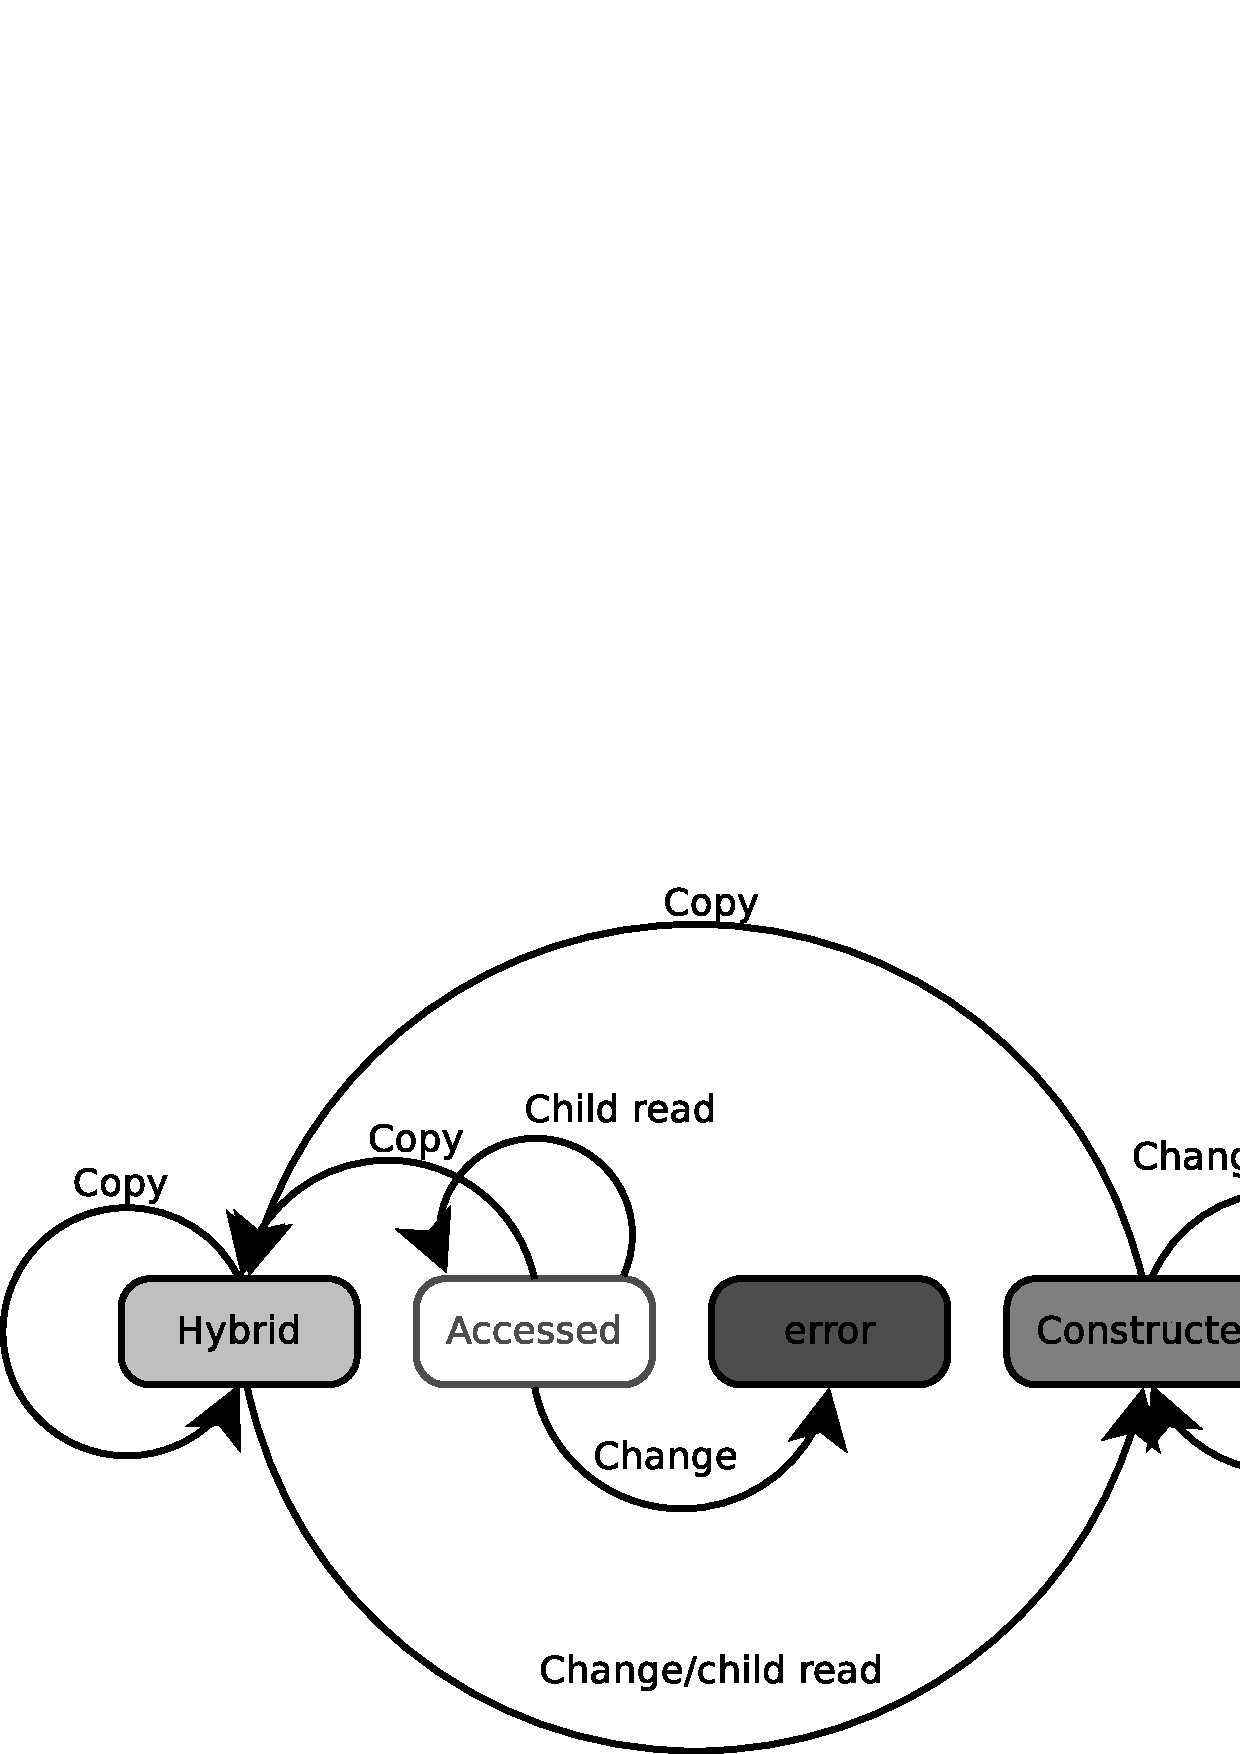
\includegraphics[scale=0.25]{hybrid_kinds_transitions}
  \caption{Node State Transitions}
  \label{fig:kinds_transitions}
\end{figure}

\begin{figure}[h]
  \centering
  \begin{code}
    \lineno <?xml version="1.0"?>\\
    \lineno <root>\\
    \lineno \><elem>elem1</elem>\\
    \lineno \><elem>elem2</elem>\\
    \lineno </root>
  \end{code}
  \caption{\texttt{doc.xml} contents}
  \label{fig:docXml}
\end{figure}


\begin{figure}[h]
  \centering
  \begin{code}
    \lineno element myroot \{\\
    \lineno \>attribute attr \{ 'value' \},\\
    \lineno \>fn:doc("doc.xml")/elem[0]\\
    \lineno \}
  \end{code}
  \caption{Example Query 1}
  \label{ex:simpleQuery}
\end{figure}
   
Consider a document {\tt doc.xml} (it's content is shown at
figure \ref{fig:docXml}) and query~1 (figure \ref{ex:simpleQuery}).
During execution of the query, following actions are performed:

    
\begin{enumerate}
    \item \label{simpleQuery::nodeCreation}
        The \texttt{myroot} element is created in a constructed state. 
        Then {\em change actions} are
        issued on that node: setting the node name ``myroot'',
        adding attribute ``attr'' and appending a text node.
    \item \label{simpleQuery::copy}
        Afterwards, the \texttt{doc.xml} is read and two {\em child read actions}
        are performed in order to evaluate XPath expression.
        %-- first on 
        %document node (which is initially in accessed state) and second on root 
        %element node (also initially in accessed state). 
    \item 
        Finally, the first \texttt{elem} (accessed) node from \texttt{doc.xml} 
        is to be added into the \texttt{myroot} (constructed) node -- the 
        \texttt{elem} node and all its descendants should be copied. 
        % --
        %the XQuery processor issue a {\em copy action} on \texttt{elem} node. 

        %Instead of doing physical (deep) copy of given node, we change its state 
        %to the hybrid state and set a ``alternate'' parent node to 
        %\texttt{myroot}. None of nodes descendants is ever touched.  
        %Effectively, hybrid nodes are temporarily shared among multiple
        %node hierarchies, as depicted at figure \ref{fig:sharedNode}.
\end{enumerate}

\subsection{Transitions}
\begin{figure}[ht]
\begin{center}
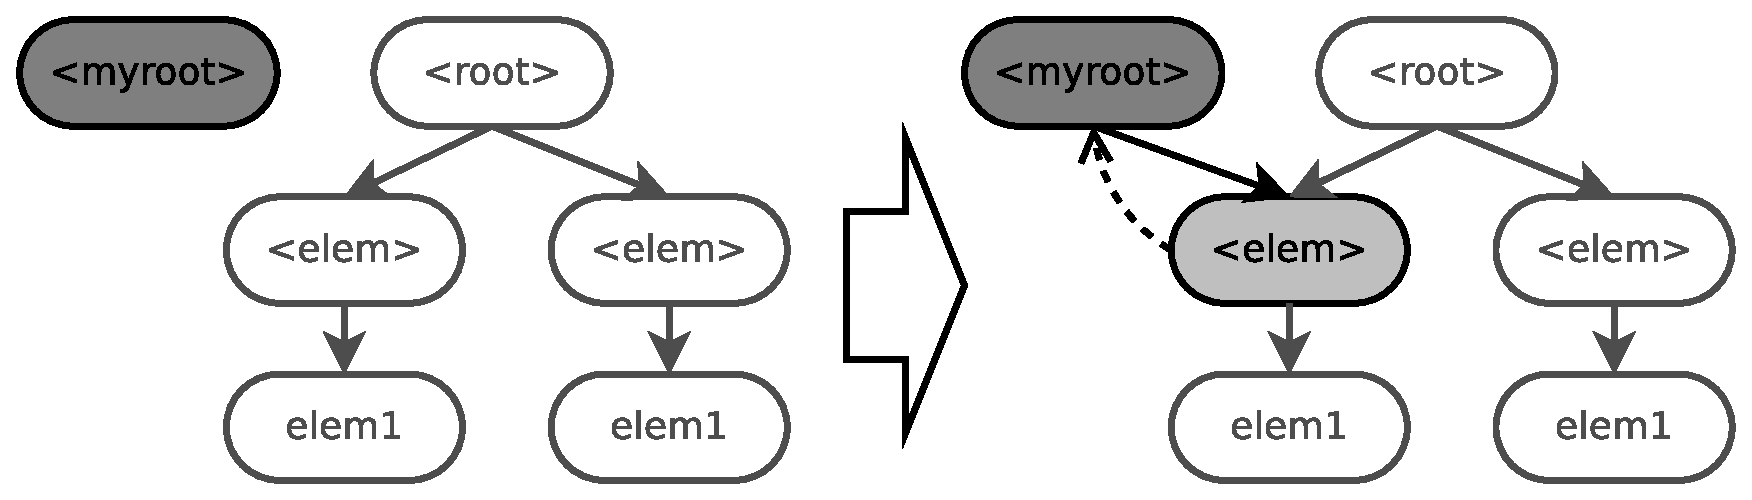
\includegraphics[scale=0.25]{shared_node}
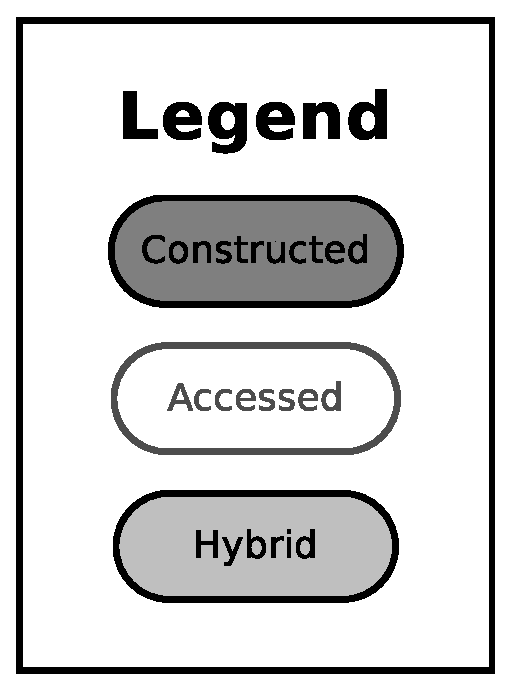
\includegraphics[scale=0.18]{legend}
\caption{Two XML trees sharing one hybrid node}
\label{fig:sharedNode}
\end{center}
\end{figure}

\subsubsection{Accessed Node Transitions.}    
    When a copy action of accessed node is triggered, the node state is 
    changed from accessed to hybrid and no physical data copy is made. 
    Changes to accessed nodes are not permitted -- any change will immediately
    lead into an error.      

\subsubsection{Constructed Node Transitions.}
    Copy operations on constructed nodes behaves exactly as on accessed nodes. 
    Changes to constructed nodes are permitted.

\subsubsection{Hybrid Node Transitions.}
    Transitions based on actions on hybrid nodes are bit more interesting:

    \begin{description}
      \item[Copy Action.] Copy action on hybrid nodes is a no-op. As a 
        result, the same node is returned with its state unchanged. 
      
      \item[Change Action.] Whenever any of node properties (dm:parent, dm:name 
        etc.) is to be changed the node state is changed to constructed and all 
        node properties are copied. 
        See the query at figure~\ref{ex:textChange}. When processing expression
        at line 5, two things happen (in that order):

        \begin{enumerate}
        \item 
            The text node \emph{``elem1''} (a result of \texttt{\$doc/elem[0]/text()}
            expression) is added to the \texttt{myroot} element. 
            States of nodes after this addition are depicted at left
            side of figure \ref{fig:hybridChange}.
        
        \item 
            Afterwards, the text node value \emph{``elem1``} has to be changed 
            to the \emph{``elem1 is the first''} because of the specification
            requirements. Obviously, the hybrid text node must be copied. The 
            XML data accessible though \texttt{\$doc} must remain unchanged.
        \end{enumerate}

      \item[Child Read Action.] 
      %  When a child read action is issued, the node state is changed to 
      %  constructed, all node properties are copied and a copy action is 
      %  performed for node children. 

       % The reason for such a behavior is the fact that the adaptor 
       % returns node ids for node-like properties and that the 
       % new (overridden) parent property value is not a part of 
       % underlying data model. 

      %  Let's have an hybrid element node \texttt{elem} that contains
      %  accessed text node \emph{``elem1''}. Suppose that 
      %  \texttt{./text()/../../..} expression is to be evaluated starting
      %  with hybrid node \texttt{elem} as the context node.
      %  Evaluation of such expression will result in repeated access to
      %  \texttt{dm:parent} property. Because the value parent property is 
      %  obtained using an XDM adaptor that operates only with node ids and 
      %  because the overridden parent value for given node is maintained 
      %  outside the primary data storage, there is no way how obtain correct 
      %  (overridden) parent.

        While appending a XML tree into a new structure, the state of a root 
        node of the appended tree is changed to hybrid, the reference from the 
        new structure is added to the hybrid. The rest of the appended tree 
        (children of the root node) are unchanged -- they don't know, that their
        parent has changed its state to hybrid. This cause serious problems
        while executing XPath commands.
        To overcome this issue, we convert hybrid node to a constructed one
        during child read action. Such a behavior is illustrated at figure    
        \ref{fig:childAxis}.
       
    \end{description}

Data are physically copied only when hybrid node is either being changed or
its children are being read. 

\begin{figure}[h]
  \centering
  \begin{code}
    \lineno let \$doc:= doc("doc.xml")\\
    \lineno return\\
    \lineno \> element myroot \{\\
    \lineno \> \> element myelem \{ \\
    \lineno \> \> \> \{ \$doc/elem[0]/text() \} is the first \} \\
    \lineno \> \> \} \\
    \lineno \> \}
  \end{code}
  \caption{Example Query 2}
  \label{ex:textChange}
\end{figure}

\subsubsection{Serialization of Result Set.} Once the query is processed, serialization
of result set may not lead into XML node copying. Because query is already processed,
no node kind transitions must be performed during serialization and thus no node copies
must be created. Obviously, if the application wants work with the result set as with
nodes in memory and wants to perform some modification on it, the result set must 
be copied. 
   
\begin{figure}[ht]
    \begin{center}
        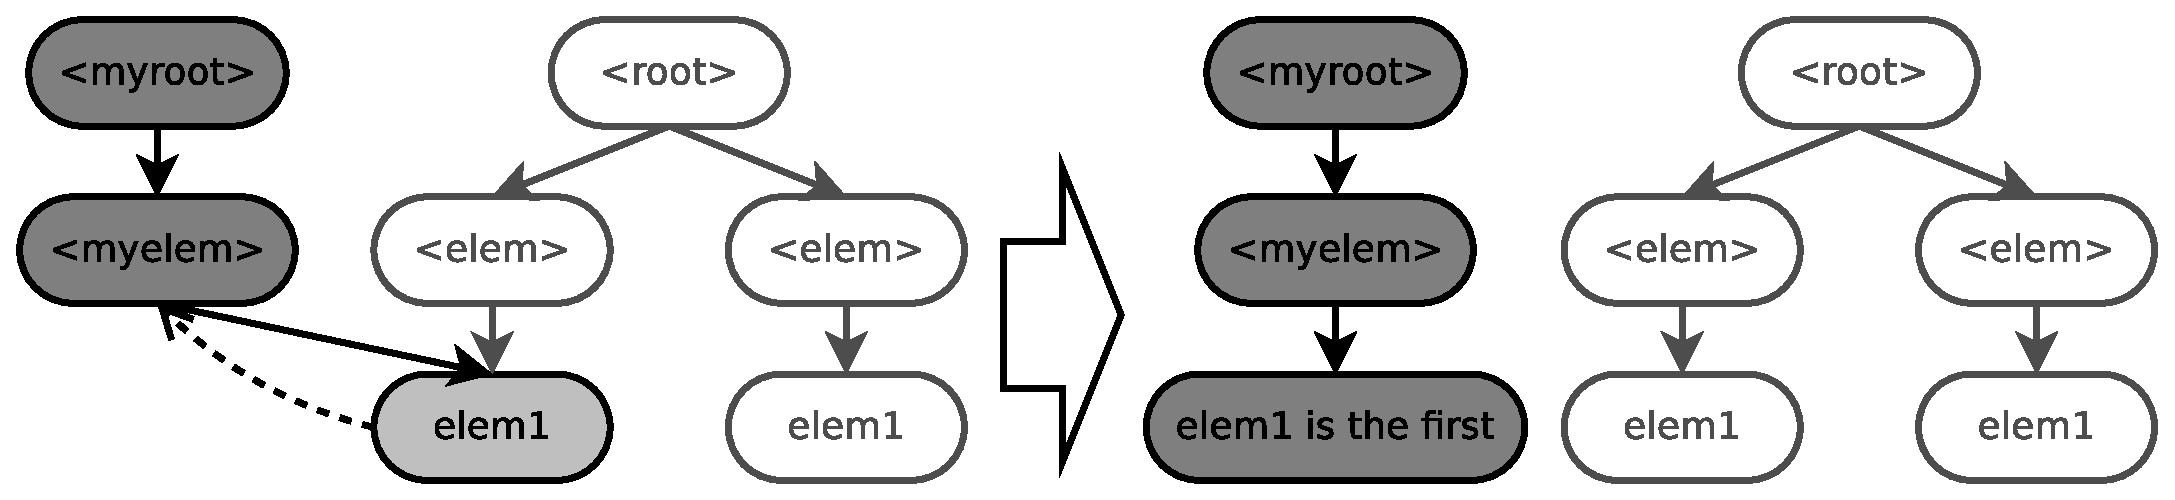
\includegraphics[scale=0.25]{hybrid_change}
        \caption{Change of hybrid node into the constructed node}
        \label{fig:hybridChange}
    \end{center}
\end{figure}

\begin{figure}[ht]
    \begin{center}
        \includegraphics[scale=0.25]{child_axis}
        \caption{Change of hybrid node while exploring the children}
        \label{fig:childAxis}
    \end{center}
\end{figure}
        

%\section{Implementation issues}
%\label{sec:impl}

%\subsubsection{XDM Adaptor.}
%    XDMAdaptor is an interface providing set of accessors as defined
%    in XDM specification \cite{xdmspec}. The whole XQuery interpretation
%    is based on the XDM interface hence the XQuery could be executed
%    over any model providing the XDM accessors.

%\subsubsection{Accessing the Document.}
%    According to the data source required in an XQuery command, the appropriate%    XDM Adaptor is selected and a XQuery is executed. There is no need to 
%     import the document to the internal XML representation. This fact allows to
%     implement deferred node copy and save copy operations and memory 
%     usage.

% \subsubsection{Strategy Pattern.}
%     In order to change the node behaviour without any impact for the XQuery
%     interpreter, the strategy pattern is used\cite{Gamm93b}. There are three strategies
%     for each node state (accessed, constructed and hybrid). According to the
%     methods called on a node object, the strategy is changed within the scope
%     of a node object without any impact for clients using the node object.

\section{Discussion}
\label{sec:discussion}

\begin{table}[ht]
\begin{center}
\tabcolsep=0.3em
\renewcommand{\arraystretch}{1.3}
\begin{tabular}{|c|r|r|r|r||c|r|r|r|r|}\hline
Q. \#& \multicolumn{2}{|c|}{\textbf{DNC}} & \multicolumn{2}{|c||}{\textbf{IC}}&
Q. \#& \multicolumn{2}{|c|}{\textbf{DNC}} & \multicolumn{2}{|c|}{\textbf{IC}}\\
    \hline
        & $N_h$ & $N_c$ & $N_h$ &$N_c$  &
        & $N_h$ & $N_c$ & $N_h$ &$N_c$  \\
	\hline\hline
	Q1  & 0          & 0     & 0          & 0     &
	Q2  & 106        & 0     & 0          & 106   \\
	Q3  & 0          & 44    & 0          & 44    &
        %Bug v attributech, melo by byt 40:0:0 pri zapnute optimalizaci
	Q4  & 0          & 0     & 0          & 0     \\
        % Nejspis nejaka chyba, vysledek je prazdny\\
	Q5  & 0          & 0     & 0          & 0     &
	Q6  & 0          & 0     & 0          & 0     \\
	Q7  & 0          & 0     & 0          & 0     &
	Q8  & 25	     & 25    & 0          & 50    \\
	Q9  & 12	     & 25    & 0          & 39    &
	Q10 & 402	     & 1     & 0          & 1244  \\
	Q11 & 12	     & 25    & 0          & 39    &
	Q12 & 3          & 3     & 0          & 6     \\
	Q13 & 22	     & 22    & 0          & 560   &% Zase chyba jak v Q3\\
	Q14 & 0          & 0     & 0          & 0     \\
	Q15 & 7          & 0     & 0          & 7     &
	Q16 & 0          & 6     & 0          & 6     \\% Stejna chyba jak Q3\\
	Q17 & 0          & 138   & 0          & 138   &% Stejna chyba jak Q3\\
	Q18 & 0          & 0     & 0          & 0     \\
	Q19 & 217	     & 217   & 0          & 434   &% Stejna chyba jak Q3\\
	Q20 & 8          & 0     & 0          & 12    \\
    \hline
    INC
        & 2074  & 114   & 0          & 5857  &
    \multicolumn{5}{|c|}{}                              \\
	\hline
\end{tabular}
\end{center}
Legend:
\begin{description}
\item[$N_h$] -- number of hybrid nodes created
\item[$N_c$] -- number of physically copied nodes
\item[DNC] -- evaluated using deferred node-copying scheme
\item[IC] -- evaluated using immediate copy as specified by the XQuery specification
\end{description}
\begin{center}
\label{tab:benchRes}
\caption{Benchmark results}
\end{center}
\end{table}

\subsection{Specification Conformance}

Although deferred node-copying scheme does not require the XML nodes to
belong to exactly one node hierarchy it preserves original XQuery semantics.
Our claim is based on the results from the XQuery Test Suite \cite{XTS}.

The \textit{axes tests} and \textit{element constructors tests} from 
\textit{Minimal Conformance - Expressions} section of XQTS Catalogue
cover the node identity semantics and were used to test the correctness
of deferred node-copying scheme. Our proof-of-concept implementation
successfully passes all the mentioned test cases.


\subsection{Benchmarks}

Presented deferred node-copying scheme has been developed 
in order to increase XQuery processor performance by reducing number 
of copy operations. 
A natural question is whether this scheme has substantial effect in
real-world applications. The table \ref{tab:benchRes} shows number of copy 
operations for selected XMark \cite{Schmidt02a} queries\footnote{Plus one 
nonstandard query marked INC. Its code
is \texttt{element a \{doc("file:///auctions.xml") \}}. We include it as an
illustration of extreme case.} on a file created with 
the XMark data generator.



Number of saved copies is dependent on a query characteristics. There are no new
nodes created in a Q1 command and that is why there is no difference in results.
There are text nodes appended to elements in a Q2 command. The text nodes does 
not need to be copied at all, only transformed to the hybrid state.

There is a subtree appended to each result item during the Q13 execution. 
Without the optimization, each element of a tree has to be copied, but with
the optimization turned on, only a few of nodes are copied. 
    
\section{Related Work}

\subsubsection{eXist XQuery Processor.}
eXist\footnote{http://exist.sourceforge.net/} is an open-source XML-native
database with XQuery as its primary query language. As far as we know, 
eXist XQuery implementation unconditionally copies nodes whenever 
the node is to be added into a different node hierarchy. Our approach is 
different since we avoid unnecessary copy operations. 

\subsubsection{Saxon XQuery Processor.}
\label{sec:related}
Saxon\footnote{http://saxon.sourceforge.net/} is well-known, widely adopted XML tool set including XSLT 2.0, XPath 2.0
and XQuery 1.0 processor. Saxon's XQuery processor introduces concept of
{\em virtual nodes} -- a light-weigh node shallow copies that shares as many properties
as possible with their origin. 

Similarly to our approach, for a given virtual node some of standard XDM properties 
may be overridden  -- namely the parent property. When the Saxon XQuery processor
iterates over virtual node's children, those are converted to virtual nodes.

However, presented deferred node copying scheme differs from 
virtual nodes approach in several aspects: 
\begin{enumerate}
  \item 
    Creating virtual copies requires a new object to be allocated
    in the memory. Deferred node copying scheme shares the same object.
  \item   
    Creation of virtual copies is a part of XQuery processing logic
    and must be explicitly expressed, whereas our approach separates
    copying logic of an XDM model from the query evaluation logic. 
%  \item   
%    Saxon's approach requires whole document to be present
%    in the memory. Our approach introduces yet another level of laziness:
%    due to the existence of XDM adapters, parts of the
%    XDM model might be loaded on demand and/or discarded when not needed
%    without breaking the XQuery semantics. Moreover, such a lazy
%    loading of XML data from primary storage is also well separated
%    from the XQuery processing logic. 
\end{enumerate}

\section{Conclusion and Future Work}
\label{sec:conclusion}

This paper presents a deferred XML node-copying scheme for XQuery
processors that significantly reduces number of source nodes copy 
operations required during query processing. This scheme defers the copy
operation unless absolutely inevitable. Whether the node is actually 
copied depends on a node state, a new property which is 
maintained for each node in addition to standard XDM properties. 
Correctness of this approach has been successfully tested by 
XQuery Test Suite. 

The main benefits of deferred node-copying scheme are: 
(i) efficiency, (ii) easy to implement, (iii) independent on
physical data model and (iv) independent on XQuery processing
logic.

As a future plan, we plan to extend this scheme for use with
various XML indexing approaches, Ctree \cite{Zou04a} and
\cite{Zou04b} in particular.

%{\bf Acknowledgement.} \todo{ask MV}
                     
\bibliographystyle{abbrv}
\bibliography{references}

\end{document}

